\section{Installation}
\subsection{System Requirements}
Before installing or compiling \gretlpy, please ensure
the following components are installed:
\begin{itemize}
	\item One of the supported versions of \python: (\reqpython);
	\item The following required \python packages: \pkg{csv},
		\pkg{json}, \pkg{numpy}, \pkg{pandas}, and \pkg{subprocess};
	\item \gretl (refer to \url{https://gretl.sourceforge.net} for details)%
		\footnote{Note: For MS Windows, the UCRT build is required. See:
			\url{https://sourceforge.net/projects/gretl/files/snapshots/}.};
\end{itemize}

\subsection{Native MS Windows}
The easiest way to install \gretlpy on a Windows machine is
by running the \installbat script from the \gretlpy root
directory. The script assumes that \texttt{python.exe} is
available in the current \texttt{PATH}. If this is not the case,
please modify \installbat accordingly. Additionally, the script
assumes that \gretl is installed in the default location, i.e.,
\texttt{C:\textbackslash Program Files\textbackslash gretl}. If
this is not the case, please modify \texttt{gretl4py\_env.bat}
or \texttt{gretl4py\_env.ps1} as needed.

The \installbat script will copy the following files into the
path generated by the command: \texttt{python.exe -m site --user-site}:

\begin{itemize}
	\item \texttt{\_\_init\_\_.py}, \texttt{gretl4py\_addons.py},
		and \texttt{gretl4py\_classes.py} from the \texttt{[gretl]} directory;
	\item \texttt{\_gretl.cp3xx-win\_amd64.pyd} from the
		\texttt{[builds\textbackslash win64\textbackslash 3.xx]} directory;
	\item \texttt{glib-2.0.dll} and \texttt{libintl-8.dll} from the
		\texttt{[builds\textbackslash win64\textbackslash DLL]} directory%
		\footnote{This is a temporary solution, and the copying of these
			two files will be removed in a future update.};
\end{itemize}

In this context, \texttt{3.xx} refers to the version of \python being used.
Figure~\ref{fig:mswindows_install.bat} shows an example output from \installbat.

\begin{figure}[h]
	\centering
	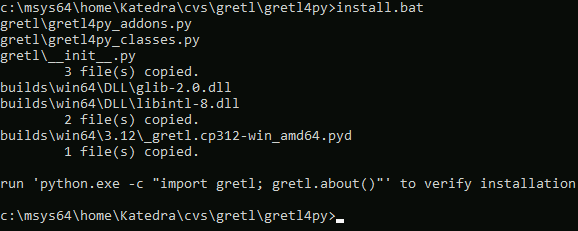
\includegraphics[width=.75\columnwidth,keepaspectratio]{mswindows_install.bat}
	\label{fig:mswindows_install.bat}
	\caption{Example output from \installbat}
\end{figure}
